\begingroup
\renewcommand{\normalsize}{\fontsize{11.1pt}{13.3pt}\selectfont}
\normalsize
\section{Question 3: Fixed-Split Cross-GPU Substitution}
\label{sec:q3}

\subsection{Model and assumptions}
We study a finite, whole-card, pre-start substitution policy on the supplied trace of 224,112 jobs. Job $j$ has native GPU model $n_j$, actual execution model $m_j$, duration $p_j$, worker count $W_j$, per-worker GPU request $g_j$, and per-worker CPU request $c_j$. A compatibility indicator $K_{jm}$ and multiplier $\sigma_{jm}$ are declared scenario assumptions; they are not measured hardware facts. For the only foreign edge in this study, A10 jobs may execute on A100-SXM4-80GB and
\begin{equation}
 p'_j=\sigma_{jm}p_j,
 \qquad f_j=s_j+p'_j,
 \qquad \omega_j=s_j-a_j.
\end{equation}
The fixed partition reserves the first $B$ A100 nodes in ascending `node_name` order for routed A10 jobs and leaves the other A100 nodes for native A100 jobs. Each worker's CPU and GPU remain on one physical node, all workers of a job start together, jobs are non-preemptive and non-migrating, and no resource may be used twice. At every node $i$ and time $t$,
\begin{equation}
 \sum_{j:s_j\le t<f_j}g_jy_{ji}\le G_i^{\rm cap},\qquad
 \sum_{j:s_j\le t<f_j}c_jy_{ji}\le C_i^{\rm cap},\qquad
 \sum_i y_{ji}=W_j.
\end{equation}
The model is a deterministic scheduling heuristic, not an optimality claim.

\subsection{Fixed-split counterfactual design}
M0 is the original model-isolated schedule. S0 is the earlier Q3-S1 M1 result, renamed to make the comparison unambiguous: 60 dedicated A100 nodes, a 10\% SHA-256 threshold, and $\sigma=1$. S1--S5 vary exactly one factor from S0: 5\% or 20\% routing, 30 or 90 donor nodes, or $\sigma=2$. The hash namespace is fixed as `q3-fixed-split-v1`; eligibility uses only the current job and declared capacity. There is no fallback from the foreign queue and no relocation of a running job.

We report $W=s-a$, actual JCT $J=f-a$, relative completion delay $f-a-p_j$, and paired finish difference $f_{\rm scenario}-f_{\rm reference}$. Every comparison uses the same original job IDs. The 90-day window is $H=7,776,000$ seconds; waiting and JCT use complete drain, while completion counts use $f_j\le H$.

\begin{table}[!ht]
\centering
\caption{Main Q3 results generated from the paper-ready JSON. Native harmed counts are paired against S0 under the same policy.}
\label{tab:q3_main}
\scriptsize
\begin{tabular}{llrrrrrr}
\toprule
Scenario & Policy & A10 $\bar W$ (h) & A10 P95/P99 (h) & A10 $\bar J$ (h) & Native harm & All $\bar J$ (h) & 90d done \\
\midrule
M0 & FCFS & 900.129 & 1408.478/1419.616 & 999.898 & 0 & 523.961 & 165,107 \
S0 & FCFS & 587.875 & 966.761/987.569 & 687.645 & 0 & 368.910 & 181,112 \
S1 & FCFS & 702.551 & 1167.986/1188.658 & 802.320 & 0 & 425.853 & 174,693 \
S2 & FCFS & 1010.136 & 4322.906/5345.115 & 1109.905 & 0 & 578.586 & 177,498 \
S3 & FCFS & 916.407 & 4053.782/4423.899 & 1016.177 & 0 & 532.044 & 174,139 \
S4 & FCFS & 539.109 & 958.246/985.841 & 638.878 & 5,735 & 344.723 & 184,339 \
S5 & FCFS & 721.752 & 2292.733/2885.707 & 831.456 & 0 & 440.320 & 177,166 \
M0 & SJF-HOL & 32.906 & 11.087/1542.181 & 132.676 & 0 & 93.353 & 217,570 \
S0 & SJF-HOL & 20.534 & 12.691/639.532 & 120.303 & 0 & 87.209 & 217,814 \
S1 & SJF-HOL & 25.328 & 7.745/1108.877 & 125.097 & 0 & 89.589 & 217,766 \
S2 & SJF-HOL & 22.058 & 9.767/526.165 & 121.827 & 0 & 87.965 & 218,104 \
S3 & SJF-HOL & 25.565 & 11.470/1025.261 & 125.334 & 0 & 89.707 & 217,762 \
S4 & SJF-HOL & 19.214 & 5.205/611.002 & 118.984 & 2,150 & 86.560 & 217,945 \
S5 & SJF-HOL & 25.106 & 12.125/1058.270 & 134.810 & 0 & 94.412 & 217,521 \
\bottomrule
\end{tabular}

\end{table}

\subsection{Benefit, native-pool cost and sensitivity}
With $\sigma=1$, S0 reduces A10 mean waiting from 900.129 to 587.875 hours under FCFS (34.7\% relative to M0) and from 32.906 to 20.534 hours under SJF-HOL (37.6\%). Cluster-wide mean JCT changes from 523.961 to 368.910 hours for FCFS and from 93.353 to 87.209 hours for SJF-HOL. The native A100 mean and P99 waiting costs are zero in S0 on this trace; this is a trace result, not an SLA.

More routing is not uniformly better. At 60 donor nodes, FCFS A10 mean waiting is 702.551, 587.875, and 1010.136 hours at 5\%, 10\%, and 20\%. The 20\% case is worse than both 10\% and M0. SJF-HOL gives 25.328, 20.534, and 22.058 hours, while its P99 tail and 90-day completion count move differently. These are finite fixed-split observations; they do not establish monotonicity for another trace or a dynamic policy.

At 10\% routing and $\sigma=1$, increasing donors from 30 to 60 to 90 lowers A10 mean waiting for both policies, but 90 nodes creates native A100 harm: 5,735 FCFS jobs and 2,150 SJF-HOL jobs wait longer than in S0. Their mean additional waits are 0.0771 and 0.0185 hours, respectively. The 90-node point remains in the trade-off table rather than being discarded.

\begin{figure}[!ht]
\centering
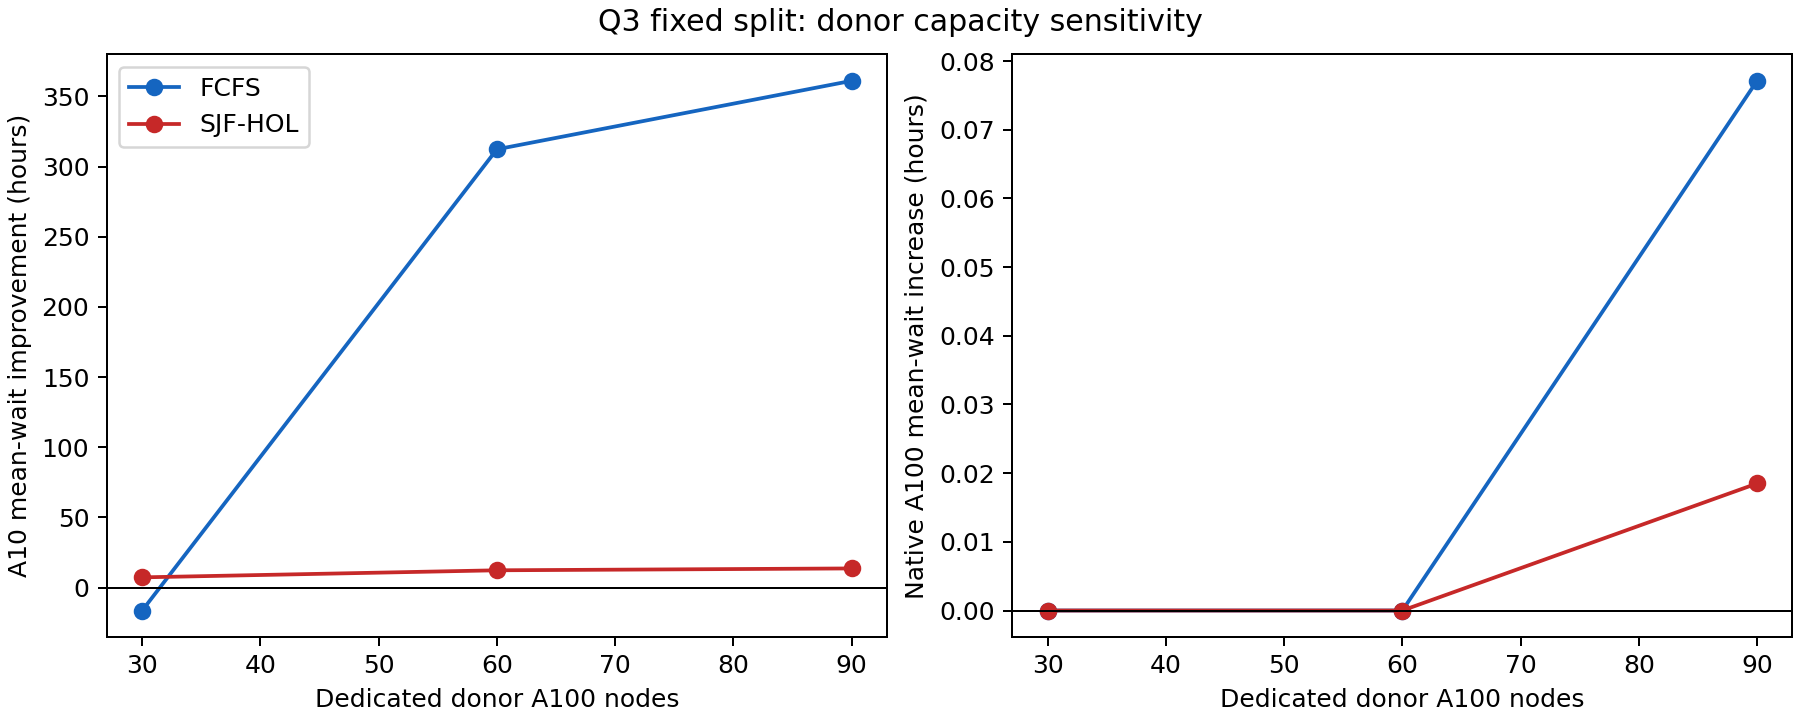
\includegraphics[width=\textwidth]{figures/q3_donor_capacity_wait_tradeoff.png}
\caption{Capacity sensitivity from the persisted S2 results. The left panel shows A10 mean-wait improvement relative to M0; the right panel shows native A100 mean-wait increase relative to M0. The two panels use different scales so the small native cost remains visible without being treated as zero.}
\label{fig:q3_capacity}
\end{figure}

For $\sigma=2$, the effective duration of routed A10 jobs doubles and SJF-HOL is re-simulated because its queue key changes. FCFS A10 mean JCT changes from 999.898 to 831.456 hours (paired delta -168.443 hours), while SJF-HOL changes from 132.676 to 134.810 hours (paired delta 2.134 hours). For the full trace, SJF-HOL all-job mean JCT changes from 93.353 to 94.412 hours and 90-day completions from 217,570 to 217,521; waiting falls relative to M0 but completion worsens. FCFS retains a mean-JCT benefit in this $\sigma=2$ scenario. No interpolation or exact break-even $\sigma^*$ is claimed.

\subsection{Conditional recommendation and limitations}
If the policy requirement is zero additional native A100 waiting on this trace, 60 nodes at 10\% is a tested candidate for either policy; it is not a proven maximum safe capacity or a global optimum. If a small native cost is acceptable, 90 nodes supplies an additional point on the A10--native trade-off. SJF-HOL's lower mean waiting does not remove its tail and completion-fairness losses; all harmed-job counts and positive delay totals remain in the paired evidence.

Compatibility and $\sigma$ are assumptions without an A10/A100 performance matrix. Allocation rates are request occupancy, not measured utilization; GPU-hours across models are not interchangeable compute or monetary units. The experiment adds no physical GPUs, does not implement dynamic sharing, MIG, pricing, RL, migration, or Q2\,$\times$\,Q3 scheduling, and does not prove heuristic optimality. Q1's A10 lower bound is not transferred to substituted schedules. The conclusion is therefore conditional on the declared trace, partitions, hash rule, policy, and duration scenarios.
\par\endgroup
